\documentclass[hidelinks, 12pt, oneside]{article}
\usepackage{bookmark}
\usepackage{graphicx}
\usepackage{hyperref}
\graphicspath{{images/}}
\usepackage[utf8]{inputenc}
\usepackage[english]{babel}
\begin{document}

 %titlepage
\thispagestyle{empty}
\begin{center}
\begin{minipage}{0.75\linewidth}
    \centering
    
 {\normalsize Project Tender\par}
 \vspace{1cm}
%Thesis title
    {\uppercase{\Large Project Name: Project Storm.\par}}
   	{\Large Client: Dr Linda Marshall and Ms Vreda Pieterse\par} 
    \vspace{1cm}

%Thesis title
    {\uppercase{\Huge Group Name\par}} 

%Author's name
    {\Large Rendani Dau 13381467\par}
    {\Large Elana Kuun 12029522\par}
    {\Large Semaka Malapane 13081129 \par}
    {\Large Antonia Michael 13014171\par}
    {\Large Isabel Nel 13070305\par}
    \vspace{1cm}
    
\end{minipage}
\end{center}
\clearpage

\tableofcontents
\newpage

\section{The Team}

\subsection{Antonia Michael}
 

\begin{figure}[ht!]
  \centering
    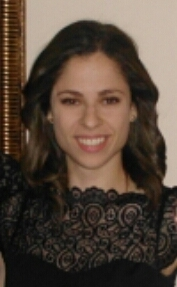
\includegraphics[width=0.85\textwidth]{t} 
\end{figure}

\subsubsection{Interests}
My interests include working with people, helping people, reading, tennis, greek dancing and spending time with family and friends. 
\subsubsection{Technical Skills}
My technical skills include: Java, C++, Html5, css, php, Bootstrap, Javascript, Semantic UI, Sql, php, python,  WebGL, Latex, Github, shell script, AngularJS, NodeJS, Microsoft Office, Npm, HandleBars Server, Mongoose, Gemfury and Mocha unit testing. 
\subsubsection{Past experiences relevant for project}
Programming \\
I have done an internship at a small IT company called Lepsta (Pty)Ltd, where I worked mainly on the front end of their new systems. I was mainly responsible to implement the gui and front end functionality of their email client app called Ridicle, using AngularJS, Python, Semantic UI, and using Brackets as the platform.
I also worked on a similar email client app there.\\
I also assisted in implementing a CMS Website for small enterprise, NCC Solutions. In addition, for COS 301 I was chosen to be part of the Infrastructure Integration team to integrate the code given to us from the functional teams. We used NodeJS, RoboMongo, Mongoose, Nodemailer, Npm, Gemfury and HandleBars server for our integration. \\

Business Analysis \\
I also worked as a business analyst at Lepsta (Pty)Ltd, where my duties included firstly, requirements management - gathering, defining, analyzing and documenting business and functional requirements and designing a solution based on these requirements. Secondly, communicating requirements to programmers and other stakeholders ensuring that everyone understands what is required for the project to be a success. I also had to develop the business processes to provide a graphical flow of data, indicating the relationship between stakeholders and systems. I had to also design the test cases and implement the testing. Throughout the process I served as a communication channel, ensuring that all the teams knew exactly what was expected of them, and reported their progress and any concerns to me.
\\
Project Management \\
At Lepsta (Pty)Ltd I also worked as a Project Manager. I developed a schedule for the project completion, allocating resources to the tasks. I also had to determine resources needed to complete the different phases of the project (i.e. time, money, technologies). I used a Gannt chart to allocate time frames for the different tasks in the project. I used a SCRUM board to keep track of the progress of the different tasks and to let the project needs see a visual representation of their tasks at hand. I had to keep regular communication with management to express the programmers' concerns and progress. It was also my job to develop team spirit and make sure that each member is contributing equally to the projects. \\
 
\subsubsection{Non technical strengths}
My non technical strengths include: \\

Firstly, I am a hard working, passionate and diligent student, who gives every task I do my full attention, and strive to only deliver good quality work. I work well with teams as I always consider each members view points and I dislike disputes, hence I always feel obliged to deliver more than my share in group projects in order to not let the large group of people that are depending on my efforts down. 
\\

Leadership skills - 
 \\1.) Head of Communications in The School of IT faculty House
 \\2.) Selected by the Department of Computer Science to be a 	Infrastructure Team Leader for the module COS 301 for the implementation of The Buzz System, 
 \\3.) Was a class Representative for the module, Imperative Programming.
   
Public speaking and presentation skills - Got chosen as the best overall paper and presentation from our presentation at the 2014 ACEIE Information Science Conference held at The University of Pretoria. Was then selected by UP to present research paper at the 2014 Information Ethics Conference held at The University of Zululand, competing with students from UJ, UP and other universities. We obrained 2nd place. 
\\
Social responsibility skills - Tutored for the Basic Computer Training course (6 sessions) for underprivileged female students eager to persue IT careers.\\ 
Organised and ran a Computer Training course for members of the community at UP Mamelodi Campus with a group of 4 other students - 40 hours of community work for JCP community development module in second year \\

Debutantes Year at school (2010) – Hosted various events/ programmes to raise funds for the Phehela Day and Night Centre and assisted with other similar charities.\\,

Teaching skills - In addition, the computer literacy courses I have taught, I am currently a Tutor in the Computer Science Department at the University of Pretoria.
Other skills: 
Communication skills, team work skills and people skills.

\subsubsection{What makes you want to do the project} 
I was interested in this project because, after having to do the mini project for most of the first semester, one gets curious to find out what is happening behind the scenes. It is hence interesting to know how the groups are formed using Belbin test results, and how the Pinochio results are used. It would also be a really satisfying feeling to be able to create software that the university will be able to use, to make the "behind the scenes" of the mini project more efficient for the lecturers, and it seems like an interesting challenge.
\\

\subsection{Rendani Dau}
\subsubsection{Interests}
My interests include music, video games, hanging out with friends and any and everything related to Information Technology including but not limited to the latest technology trends and news and how technology can be used to better our everyday lives.
\subsubsection{Technical Skills}
My technical skills include: Programming skills in Java and C/C++. Web development technologies including HTML, JavaScript/jQuery, CSS, PHP, Bootstrap and NodeJS. Database programming using SQL (MySQL and Microsoft SQL) and Mongo DB. Programming in C\# including creating Windows Forms Applications, Advanced use of the .NET framework including linking databases (SQL Server, Microsoft Access, Oracle Database, etc.) to Windows Forms for CRUD functionality, creating Runtime Libraries (DLLs), creating client/server web applications with ASP.NET and creating reports with the SAP Crystal Reports plugin for Visual Studio. Also proficient with the Microsoft Office suite, Latex, XML and related technologies (XSL and DTD).
\subsubsection{Past experiences relevant for project}
I have successfully completed web development courses including COS 216 and IMY 220 which will allow me to bring the necessary web development techniques to the team. Having also participated in the COS301 Mini project, I believe the insight and experience gained from that will be useful in this project.
\subsubsection{None technical strengths}
My non-technical strengths include teamwork and communication skills which were honed by the COS301 Mini Project, thinking on my feet to solve problems and coming up with and voicing ideas.
\subsubsection{What makes you want to do the project}
Having taken part in the COS 301 mini project, I would like to bring my experience into creating a more efficient way of picking teams which will be beneficial to both the students and lecturers of the module in future. I also think it would be great for myself and my team mates to leave behind a legacy in the Computer Science Department in the form of a fully functional app that can be used in more modules that employ group work in the department.

\subsection{Elana Kuun}
\subsubsection{Interests}
Programming is a big interest, I enjoy solving complex problems and creating working systems that other people can use. My hobbies include photography, playing music, and running. I like to read and write and I enjoy hiking trails and the outdoors. I am also very interested in psychology. 
\subsubsection{Technical Skills}
Java, C++, HTML, CSS, PHP, JavaScript, XML, SQL, NodeJS, Mongoose, XQuery, JQuery
Some experience with databases, such as Neo4j, MongoDB, db4o, PostgreSQL.
\subsubsection{Past experiences relevant for project}
I have completed all my second and third year modules for my degree and believe this knowledge can assist me in this project. The COS 301 mini project has also expanded my knowledge about web development and I am currently studying an artificial intelligence module that could also be beneficial for this project.
\subsubsection{None technical strengths}
I am conscientious and work on a project until it is done. I take ownership of my work and deliver the best quality that I can. In a team I listen to the other team members and treat them with respect. I take everyone’s opinion into account, as well as voicing my own. When the situation calls for it I will take the lead. Communication is important and I do my best to keep other people up to date and follow the progress of the team. Being organised is important to me and I am always prepared. I always plan my work and stick to deadlines.
\subsubsection{What makes you want to do the project}
I was very interested and curious about how the teams were selected for the mini-project. I like anything that has to do with people and writing a program that is relevant to this is something that I would enjoy very much. The project involves web development and artificial intelligence, I enjoy both of these areas and would value the opportunity to develop such a system.
\subsection{Semaka Malapane}

\begin{figure}[ht!]
  \centering
    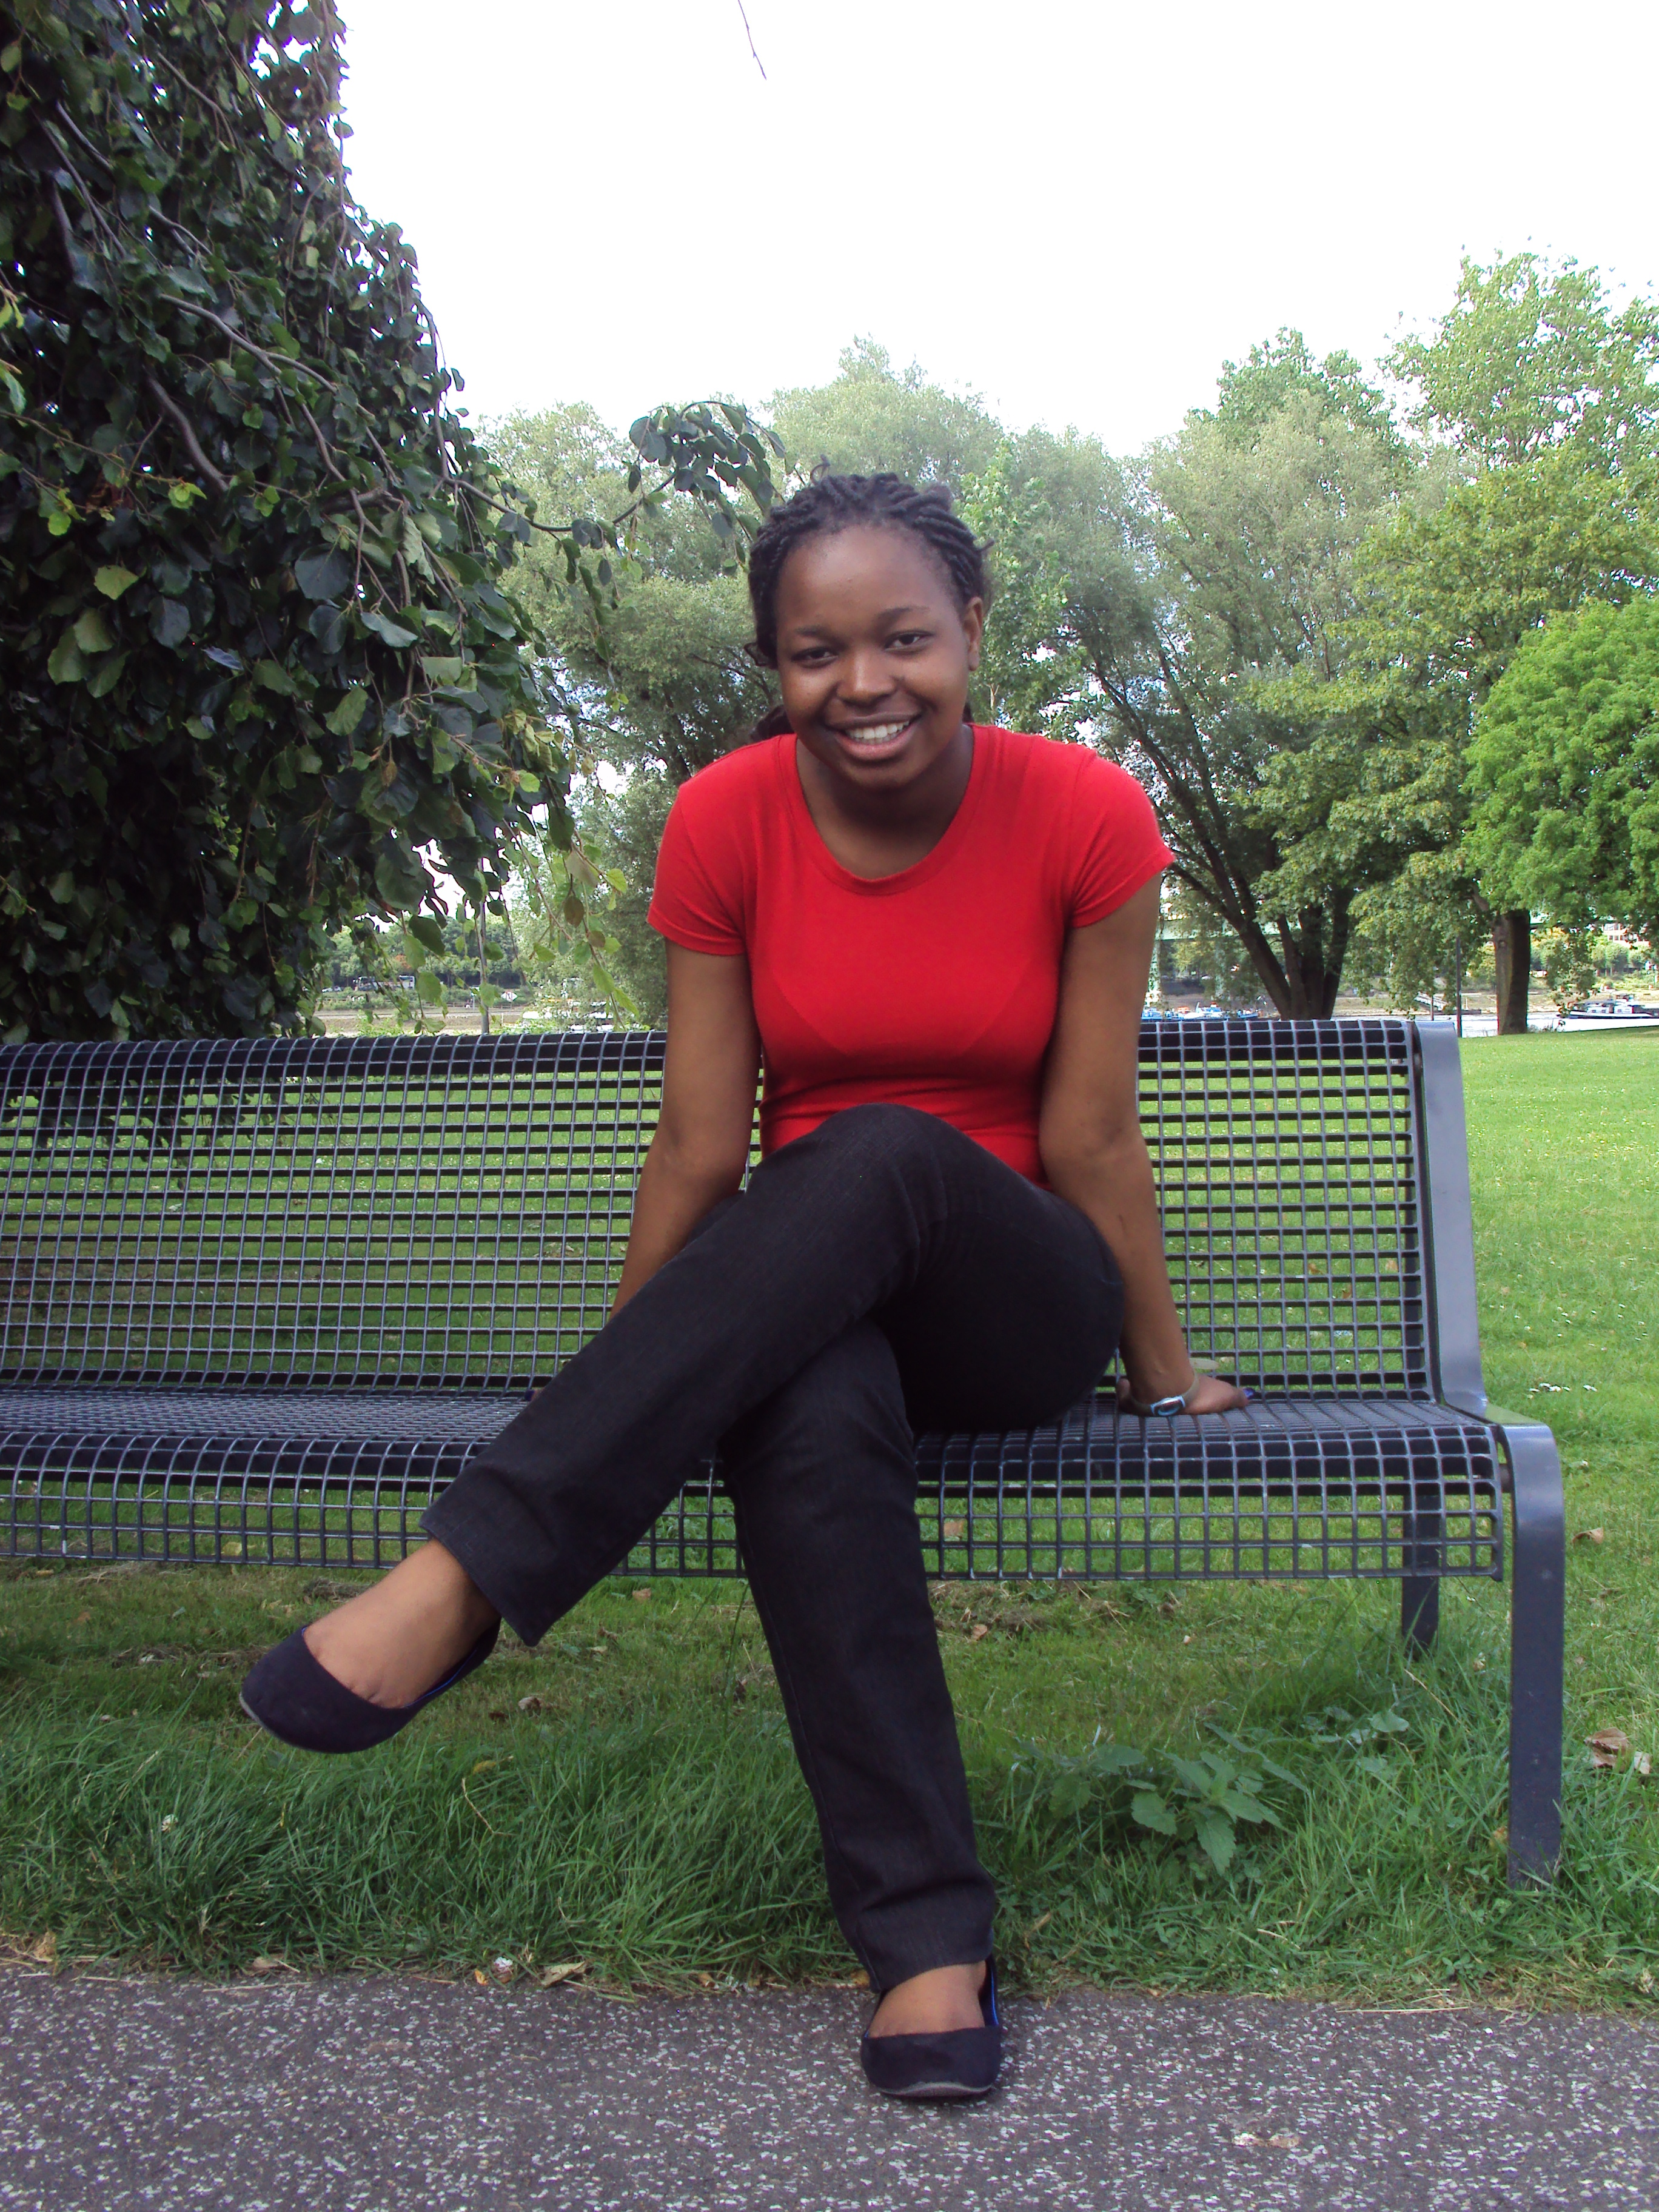
\includegraphics[width=0.85\textwidth]{Semaka} 
\end{figure}

\subsubsection{Interests}

My interests are playing sudoku, cards, puzzles, cooking, reading, shopping and spending time with friends and family.

\subsubsection{Technical Skills}

My technical skills include: C++, Java, CSS, PHP, HTML, JavaScript, NodeJS, nodeunit, Mongoose, WebGL, Microsoft Office, SQL and XML.
 
\subsubsection{Past experiences relevant for project}

I have successfully completed COS 216 (Netcentric Computer Systems)  which taught me a the required web development skills required for this project. I also believe that all the other programming modules I have done in the past two and a half years will help me and my team complete this project successfully.

\subsubsection{Non technical strengths}

My non technical strengths include: 

Team work and communication skills - The Software Engineering course offered us a mini project at the beginning of the year where we had to work in multiple different teams with different kinds of people. This gave me the opportunity to learn to work in a team setting and to communicate appropriately.
 
Public speaking and presentation skills - I participated in public speaking in 2011 and 2012. This taught me not only good speech writing but valuable presentation skills.
I also took part in a computer training course at the UP Mamelodi Campus in 2014 - this gave me the opportunity to better my public speaking and presentation skills.

Social responsibility skills - I tutored a Basic Computer Training course (6 sessions) for underprivileged female students.
I organised and ran a Computer Training course for members of the community at UP Mamelodi Campus with a group of 4 other students - 40 hours of community work for JCP community development module in second year.

\subsubsection{What makes you want to do the project}

The project sounds interesting and challenging. It is something that we will be proud of at the end of the year after having completed it.

\subsection{Isabel Nel}

\begin{figure}[ht!]
\centering
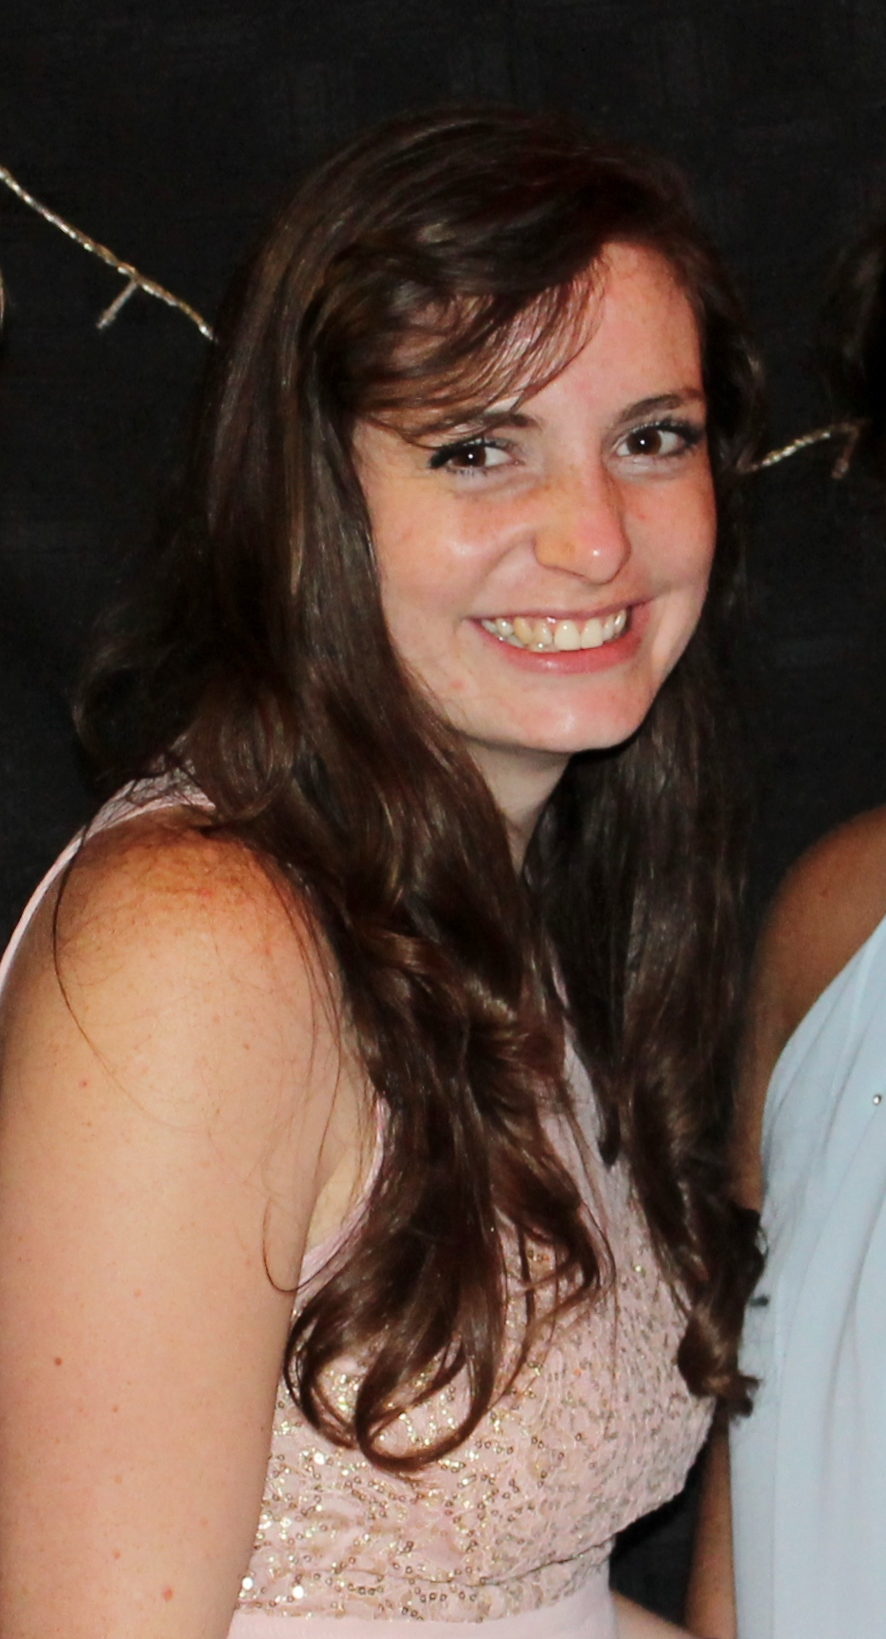
\includegraphics[width=50mm]{IsabelNel}
\end{figure}

\subsubsection{Interests}
During my past two years of studying Computer Science, I have developed a
passion for software development. Finding creative solutions to problems in
the form of software is something that denitely falls in my interests. I am
also fond of the outdoors, helping others and baking

\subsubsection{Technical Skills}
My thecnical skills include: C++, Java, CSS, PHP, JavaScript, XML, HTML,
SQL, WebGL, Micrisoft Office and NodeJS.

\subsubsection{Past experiences relevant for project}
I have successfully completed my foundational programming modules and
more specialized modules at the University of Pretoria, thus I am capable
of producing adequate and usable software. I also participated in the mini-
project of COS 301, which made use of the principles which will be used in
Project Storm, which will help with the understanding of the project.

\subsubsection{None technical strengths}
I believe I am a good team player, with that I mean that I am a supportive
person when it comes to team work, I respect my other team members and
I am good in sharing my ideas and listening to other's ideas. I can take on
a leadership position if need be, such as the position I was placed in for the
mini-project of COS 301 as a middle level team lead.

\subsubsection{What makes you want to do the project}
My previous experience with the mini-project in COS 301 is my motivation to do Project Storm. During the mini-project we were asked after each phase to fill in questions to gather information for 'Rocking the boat' and that got me thinking on how things work behind the scenes, how are group members sorted and so forth. Thus it would be interesting for me to be able to assist in the development of the software of how students are divided behind the scenes into groups according to their evaluation and personalities. 

\section{The Plan of Action}

\subsection{The development methodology we will use:}

1.) Functional requirements -  We will first formulate the use cases from the business rules given. From that we will create the services contracts and the use case diagrams (including the use case diagram for the whole system as individual components). Activity diagrams will then be drawn. Lastly, we will create the domain model for the system.

2.) Software architecture documentation - We will first devise the architectural responsibilties for the system. We will then formulate the quality requirements, with reasons that each requirement was chosen, strategies to achieve the requirement and patterns to achieve the strategies. After which the Integration requirements will be drafted. Here the integration channels, access channels, protocols and API specifications will be explained. The Architecture contraints will then be formed, including the reference architecture, technologies, and operating systems that will be used. Lastly, we will decide on which architectural patterns best fit the requirements. 

3.) Implementation phase - The use cases will be modularized and developed independantly of eachother. After thorough unit testing of the individual modules, these will be integrated into the whole system. 

4.) Testing and verification - seperate unit testing of the individual modules will be done to check if the services contracts have been followed. Automated integration testing will also be done to check that the modules only integrate with the system if their services contract has been met. 

5.) Documentation - An instruction manual with screenshots will be created as well as additional documentaion explaining the structure of the system.  

\subsection{How will you keep the client informed about the status of the project:}

We will firstly email the client at the end of each  week, stating the group's progress report from the week, we will also set up a monthly meeting with the client to demo and get feedback.  This can become a weekly meeting if required. However, we will email the client whenever we have questions or concerns.

\subsection{Any initial ideas we have around solving some of the technical challenges:}
  
\subsection{Technologies the team intends to use:} 

At this point the following technologies have been considered, but this is subject to more research and contact with the client. 

-A server provided by the CS department at UP that we have access to. 

-Sql to create and manage the databases required for access numbers the students and doctors and other databases required.

-Github for version control 
 
-Bootstrap and Semantic UI for the interface

\subsection{What the client will receive from us at the end of the project:}

A flexible, pluggable, fully functional software application  that will be maintainable, with detailed supporting documentation and an instruction manual.

 
\end{document}
